\documentclass[tikz,border=2pt]{standalone}
\usepackage{amsmath,amssymb}
\usepackage{tikz}

\begin{document}
% Inclusion-exclusion for three events: adding P(A)+P(B)+P(C) counts the pairwise overlaps
% twice and the triple overlap three times; subtract the pairs, then add the triple back.
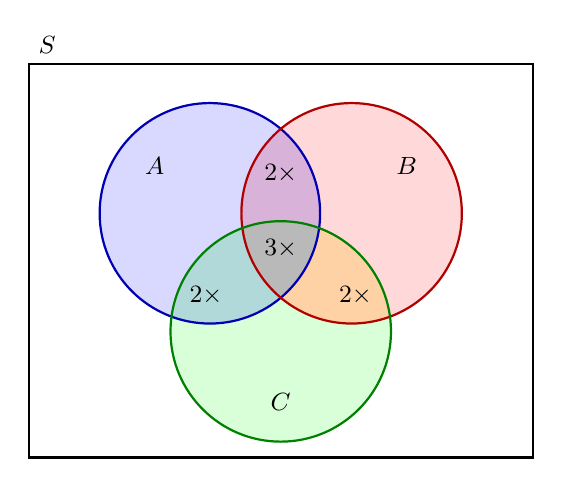
\begin{tikzpicture}[every node/.style={font=\small}]
	\draw[thick] (-3.2,-2.6) rectangle (3.2,2.4);
	\node[anchor=south west] at (-3.2,2.4) {$S$};
	\fill[blue!15] (-0.9,0.5) circle (1.4);
	\fill[red!15] (0.9,0.5) circle (1.4);
	\fill[green!15] (0,-1.0) circle (1.4);
	\begin{scope}
		\clip (-0.9,0.5) circle (1.4);
		\fill[violet!30] (0.9,0.5) circle (1.4);
		\fill[teal!30] (0,-1.0) circle (1.4);
	\end{scope}
	\begin{scope}
		\clip (0.9,0.5) circle (1.4);
		\fill[orange!35] (0,-1.0) circle (1.4);
	\end{scope}
	\begin{scope}
		\clip (-0.9,0.5) circle (1.4);
		\clip (0.9,0.5) circle (1.4);
		\fill[gray!55] (0,-1.0) circle (1.4);
	\end{scope}
	\draw[thick, blue!70!black] (-0.9,0.5) circle (1.4);
	\draw[thick, red!70!black] (0.9,0.5) circle (1.4);
	\draw[thick, green!50!black] (0,-1.0) circle (1.4);
	\node at (-1.6,1.1) {$A$};
	\node at (1.6,1.1) {$B$};
	\node at (0,-1.9) {$C$};
	\node at (0,1.0) {$2\times$};
	\node at (-0.95,-0.55) {$2\times$};
	\node at (0.95,-0.55) {$2\times$};
	\node at (0,0.05) {$3\times$};
	
\end{tikzpicture}
\end{document}
